\documentclass[12pt,pdftex,16x10]{elpres} %for wide-screen slides
%\documentclass[11pt,pdftex,4x3]{elpres} %for standard 4:3 slides

\usepackage[slides]{resources/research18}
\usepackage{subcaption}

%%%%%%%%%%%%%%%%%%%%%%%%%%%%%%%%%%%%%%%%%%%%%%%%%%%%%%%%%%%% 
%%%% Footer
%%%%%%%%%%%%%%%%%%%%%%%%%%%%%%%%%%%%%%%%%%%%%%%%%%%%%%%%%%%% 
\lfoot{\parbox[l][2mm][b]{3cm}{
\includegraphics[height=4mm]{resources/isilogo_plain}}}
\cfoot{\tiny Gaspard Ulysse Fragnière}
\rfoot{\tiny\thepage}

\begin{document}

%%%%%%%%%%%%%%%%%%%%%%%%%%%%%%%%%%%%%%%%%%%%%%%%%%%%%%%%%%%% 
%%%% Title-Slide
%%%%%%%%%%%%%%%%%%%%%%%%%%%%%%%%%%%%%%%%%%%%%%%%%%%%%%%%%%%% 
\begin{titlepage}
  \centering
  \parbox{0.6\textwidth}{
\includegraphics[height=2.2cm]{resources/ethlogo_short}}
  \hfill
  \parbox{0.35\textwidth}{ 
    \mbox{}\hfill 
\includegraphics[height=1.4cm]{resources/isilogo_plain}}
  
  Master Thesis Presentation\\
  %Semester Project Presentation\\
  21 February 2023
  
  \distance{2}
  \LARGE
  \textbf{Generative Adversarial Networks for the\\
  Generation of Microphone Array Data}
  

  \normalsize
  \distance{3}
  Gaspard Ulysse Fragnière

  \distance{4}
\end{titlepage}

%%%%%%%%%%%%%%%%%%%%%%%%%%%%%%%%%%%%%%%%%%%%%%%%%%%%%%%%%%%% 
%%%%% Slides
%%%%%%%%%%%%%%%%%%%%%%%%%%%%%%%%%%%%%%%%%%%%%%%%%%%%%%%%%%%% 


\begin{psli}[Agenda]
  \textbf{TODO: remove this slide if not more insightful}
  \begin{itemize}
    \item Introduction
    \item Some Fundamentals
    \item Methods
    \item Results and Discussion
    \item Conclusion
    \item Future Works
  \end{itemize}
\end{psli}

% NEW INTRODUCTION ============================================================
\begin{psli}[Introduction: Context]
  \begin{minipage}[b][0.7\textheight][t]{0.5\textwidth}
    \centering
    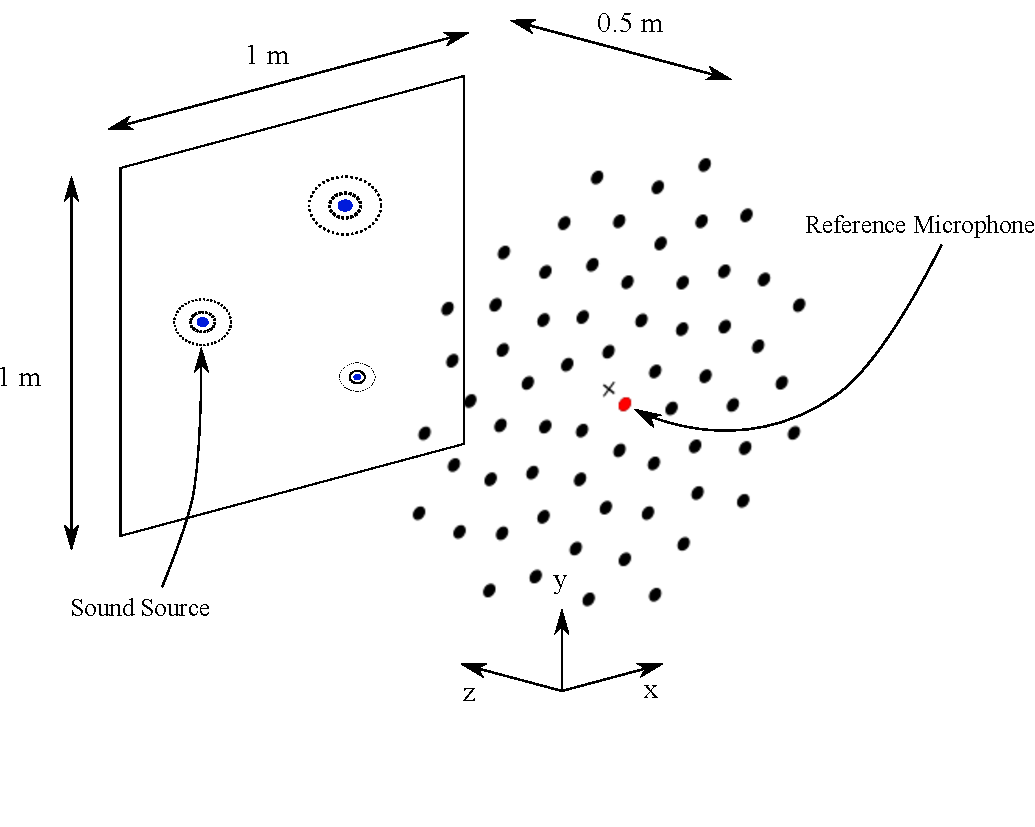
\includegraphics[width=1.1\textwidth]{figs/full_measurement_setup.pdf}
  \end{minipage}
  \begin{minipage}[b][0.7\textheight][t]{0.5\textwidth}
    \begin{itemize}
      \item Microphones array are used for source characterization.
      \item Want to create DL-based algorithm to characterize sound source (in a supervised context).
      \item Source characterization algorithm uses the Cross Spectral Matrix for stationary signal.
      \item Cross Spectral Matrix: compact representation of the microphones' signals in the frequency domain
    \end{itemize}
  \end{minipage}
\end{psli}

\begin{psli}[Introduction: Data]
  \begin{minipage}[b][0.7\textheight][t]{0.5\textwidth}
    \centering
    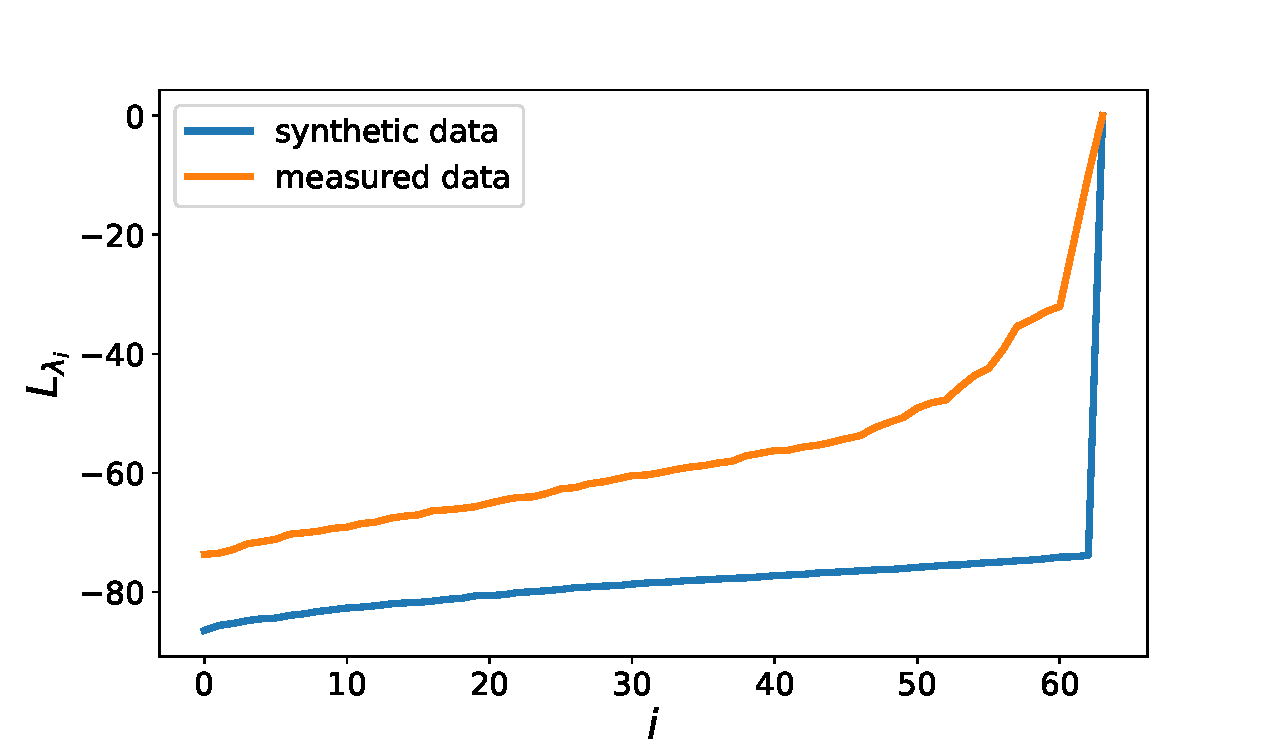
\includegraphics[width=1.1\textwidth]{figs/comparison_synthetic_measurement_data.pdf}
  \end{minipage}
  \begin{minipage}[b][0.7\textheight][t]{0.5\textwidth}
    \begin{itemize}
      \item Clear difference between measured and synthetic data
      \item Only limited amount of data for supervised learning (e.g. 50 millions sample required to train)
      \item Domain-shift
    \end{itemize}
  \end{minipage}
\end{psli}

\begin{psli}[Introduction: Generating Data ]
  
  \begin{itemize}
    \item Generative Adversarial Networks (GAN): DL-based approach to generate data
    \item Able to learn complicated data structure.
    \item Could be suited to generate realistic CSMs.
  \end{itemize}


  %https://genforce.github.io/interfacegan/assets/teaser.jpg
  \begin{figure}[h]
    \centering
    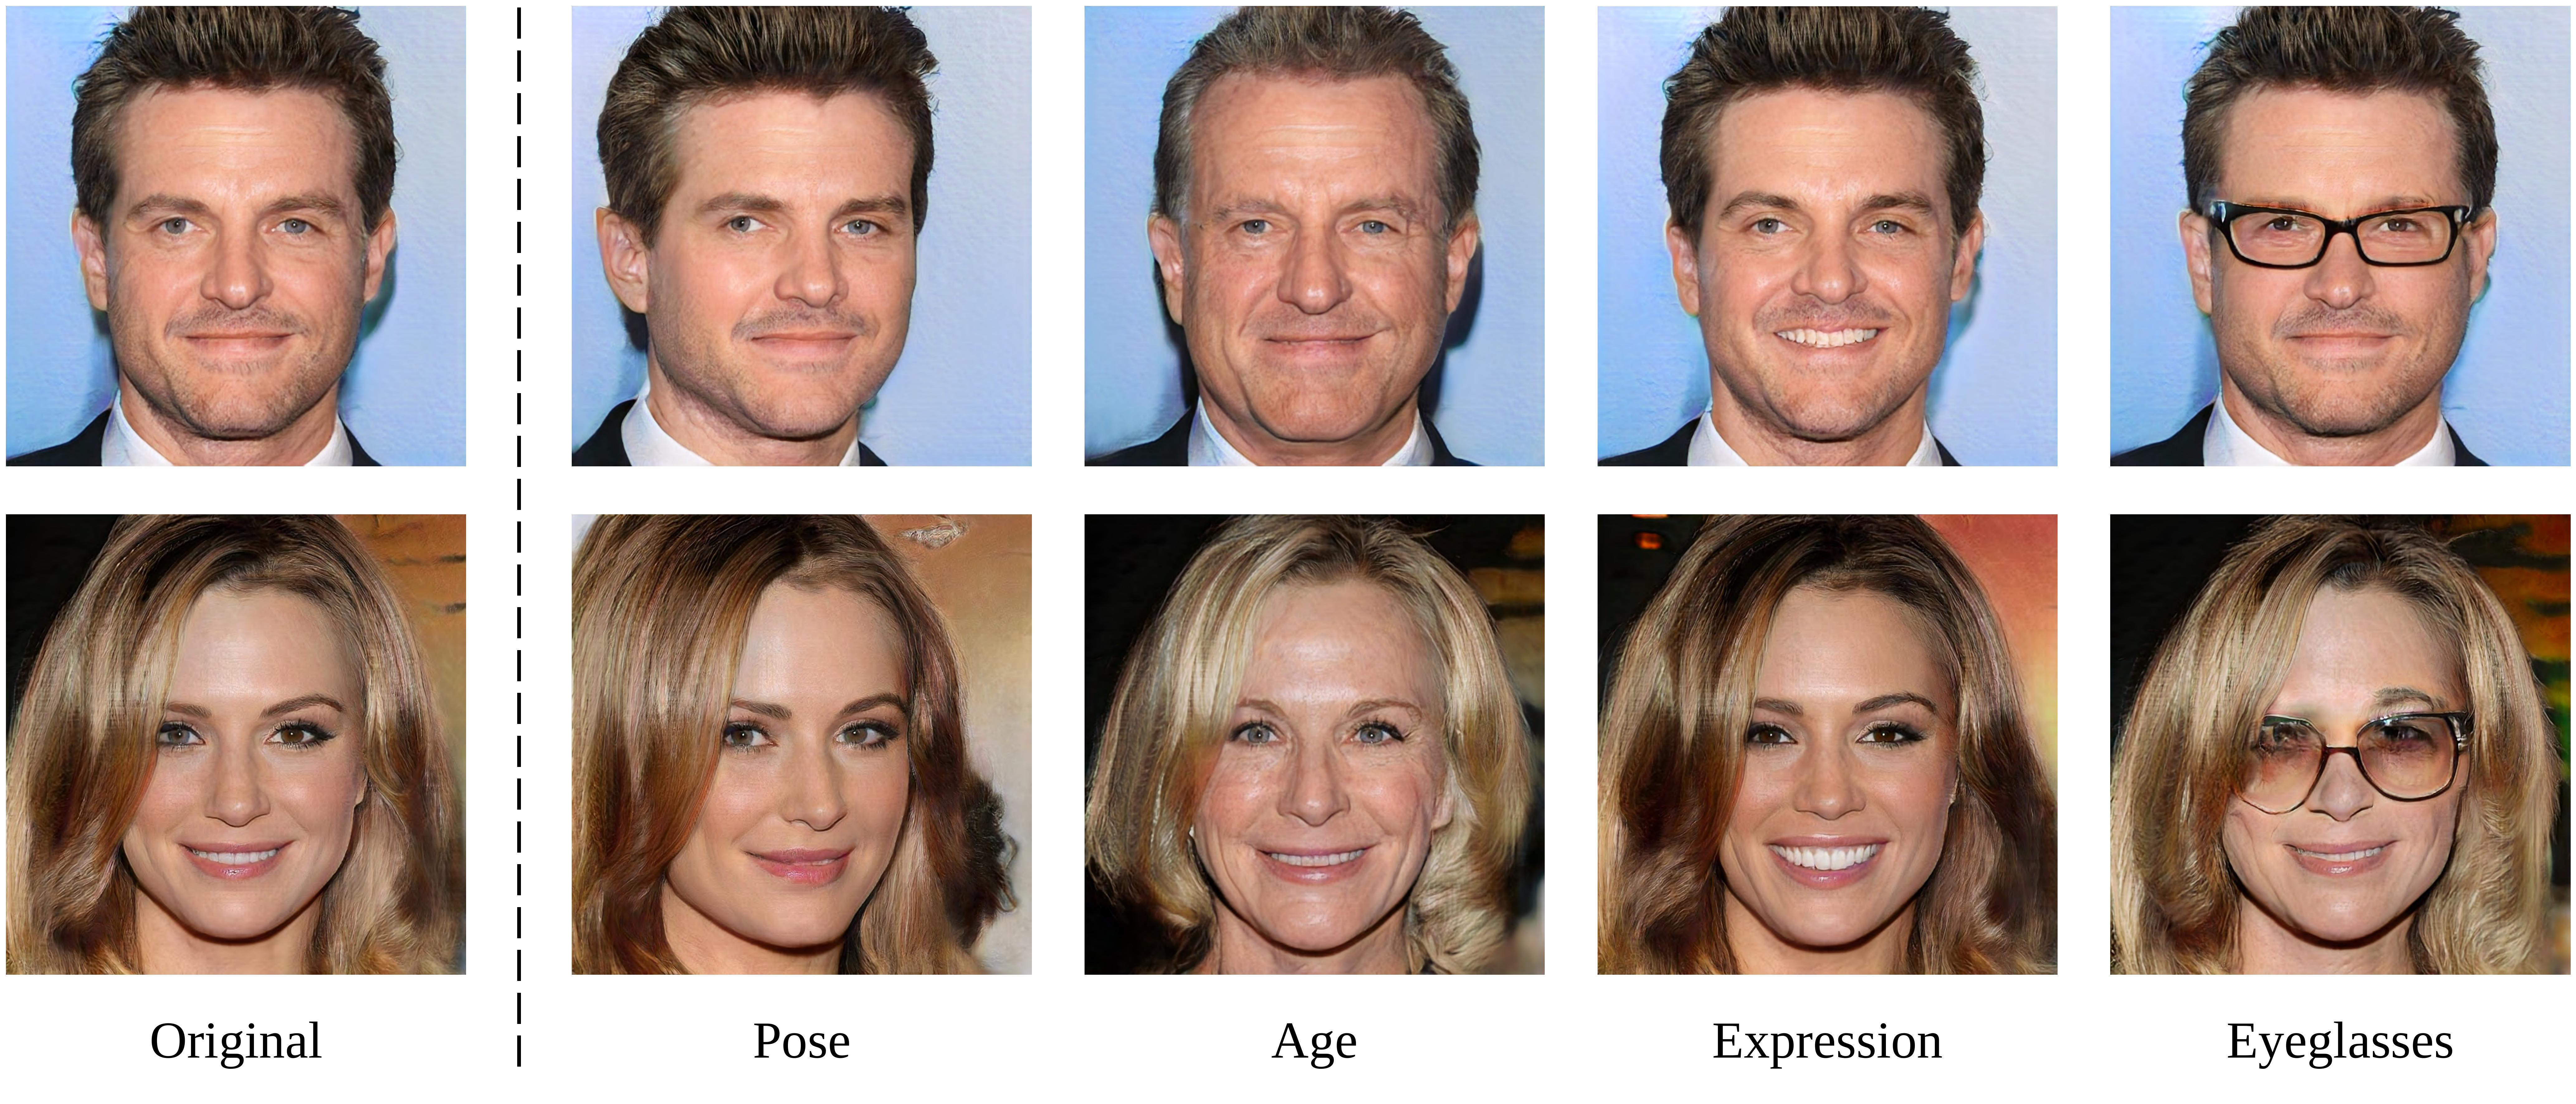
\includegraphics[width=.5\textwidth]{figs/GAN_illustration.jpg}
    \caption{Faces generated with a GAN. From \textbf{TODO: add source}}
  \end{figure}
  
\end{psli}


\begin{psli}[Introduction: Aim]
  Hence the goal of this thesis is to investigate:
  \begin{itemize}
    \item  if CSMs can be generated directly or indirectly, as realistically as possible, using a GAN approach.
    \item if training first GAN with synthetic data and fine-tune them with measurement is suited to deal with lack of data.
    \item Investigate data augmentation scheme to improve the realness of synthetic data.
  \end{itemize}
\end{psli}
% =============================================================================




\begin{psli}[Fundamentals: Sound Model]
  \begin{minipage}[b][0.7\textheight][t]{0.5\textwidth}
    \centering
    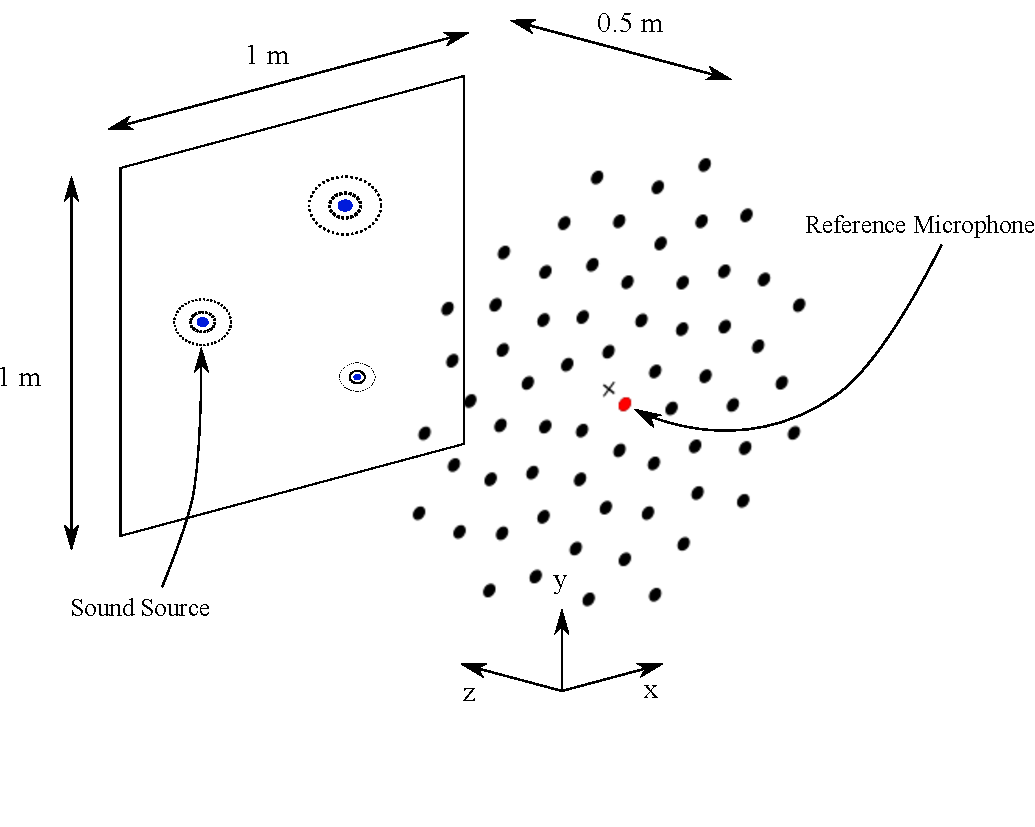
\includegraphics[width=1\textwidth]{figs/full_measurement_setup.pdf}
  \end{minipage}
  \begin{minipage}[b][0.7\textheight][t]{0.5\textwidth}
    
    The sound model equation is given by:
    \begin{equation}
        \mathbf{p} = \mathbf{H} \mathbf{q} + \mathbf{n}
    \end{equation}
    with
    
    \begin{itemize}
     \item $\mathbf{p} \in \mathbb{C}^{64}$: the pressure in the 64 microphones of the array
     \item $\mathbf{q} \in \mathbb{C}^J$: amplitudes of the $J$ uncorrelated sources
     \item $\mathbf{H} \in \mathbb{C}^{(64,J)}$: transfer function from the sources to the sensors.
     \item $\mathbf{n}$: independent noise.
    \end{itemize}
  \end{minipage}
  
\end{psli}



\begin{psli}[Fundamentals: CSM, Eigendecomposition and Rank I CSM]
  \begin{itemize}
    \item The Cross Spectral Matrix (CSM) is a representation of the sound pressure in the different microphones. Using Welch's method, it can be approximated as:

    % Mention that the CSM is used in most beamforming algorithm.
    %Welch's method applies FFT blockwise on the array time data, calculates the CSM for each time data block and finally averages the results.
    
    \begin{equation}
        \label{csm}
        \hat{\mathbf{C}} = \frac{1}{B} \sum_{b = 1}^{B} \mathbf{p}\mathbf{p}^H
    \end{equation}
    \item A Cross spectral matrix $\hat{\mathbf{C}}$ of dimension $M \times M$ can be representated by its eigenvalues and eigenvectors using:

    \begin{equation}
        \label{eigendecomposition}
        \hat{\mathbf{C}} = \mathbf{V} \mathbf{\Lambda} \mathbf{V}^H
    \end{equation}

    \item Using only one eigenvector $\mathbf{v}_i \in \mathbf{V}$ and the corresponding eigenvalue $\mathbf{\Lambda}_{ii}$, the Rank I CSM can be computed as:
    
    \begin{equation}
        \label{rank_I_csm}
        \hat{\mathbf{C}}_i = \mathbf{v}_i \mathbf{\Lambda}_{ii} \mathbf{v}_{i}^{H}
    \end{equation}
  
  \end{itemize}
\end{psli}

\begin{psli}[Fundamentals: GAN and WGAN-GP]
  \begin{itemize}
    \item GAN consists of two competing networks: generator and discriminator. 
    \item Discriminator: determine real from fake samples.
    \item Generator: produce data realistic enough to fool the discriminator.
    \item Wasserstein GAN with Gradient Penalty (WGAN-GP): improved GAN, using the  Wasserstein distance as loss function.
  \end{itemize}
  % https://towardsdatascience.com/automatically-finding-the-best-neural-network-for-your-gan-c0b97a5949f2
  \begin{figure}[h]
    \centering
    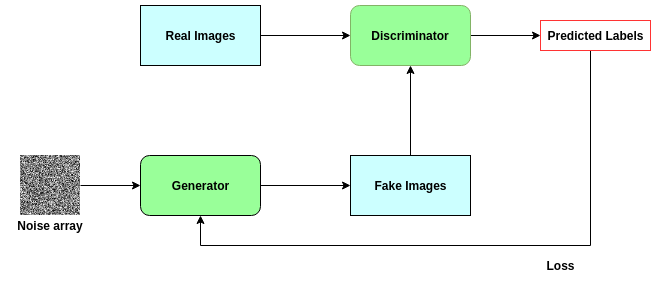
\includegraphics[width=.3\textwidth]{figs/GAN_structure.png}
    \caption{GAN Structure. From \textbf{TODO: add source}}
  \end{figure}
\end{psli}



\begin{psli}[Methods: Introduction]
  \begin{itemize}
    \item This thesis investiguates the generation of CSMs through their eigendecomposition.
    \item CSMs are complex and hermitian matrices, hence have complicated distribution to learn.
    \item Eigendecomposition is an insightful representation of source:
    \begin{itemize}
      \item Eigenvalues: represent the sources' strength
      \item Eigenvectors: represent the sources' position
    \end{itemize}
  \end{itemize}
\end{psli}

\begin{psli}[Methods: Data]
  

  \begin{itemize}
    \item Synthetic data follows a complex Wishart distribution
    \item Measurements performed with single loudspeaker in an anechoic chamber
    \item Synthetic and measurement have same position and Helmotz number $He = 16$ %which is dimensionless frequency.
  \end{itemize}

  \begin{figure}[h]
    \begin{subfigure}[b]{0.45\linewidth}
      \centering
      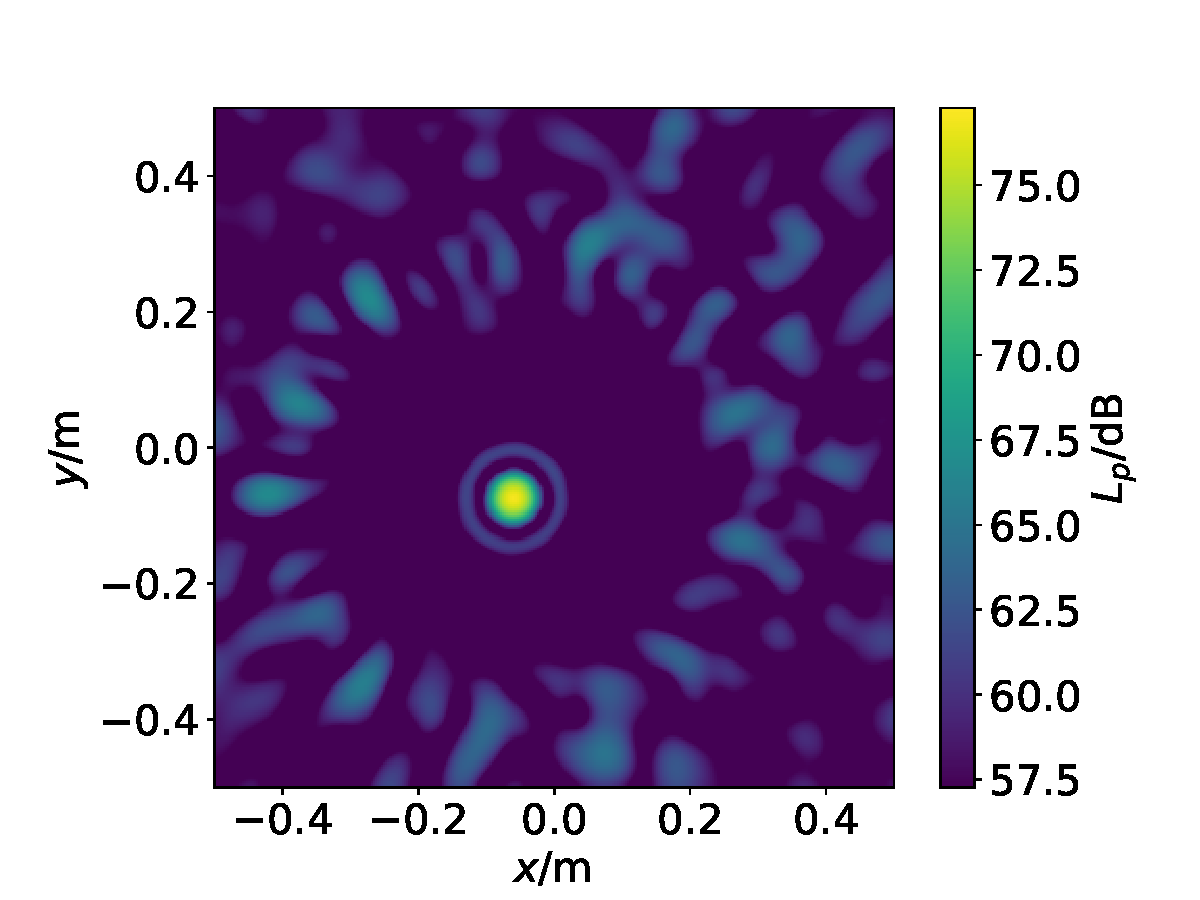
\includegraphics[width=0.75\linewidth]{figs/datasets_beamforming_example_synthetic.pdf} 
      \caption{Synthetic} 
      %\label{fig7:a} 
      %\vspace{4ex}
    \end{subfigure}%% 
    \begin{subfigure}[b]{0.45\linewidth}
      \centering
      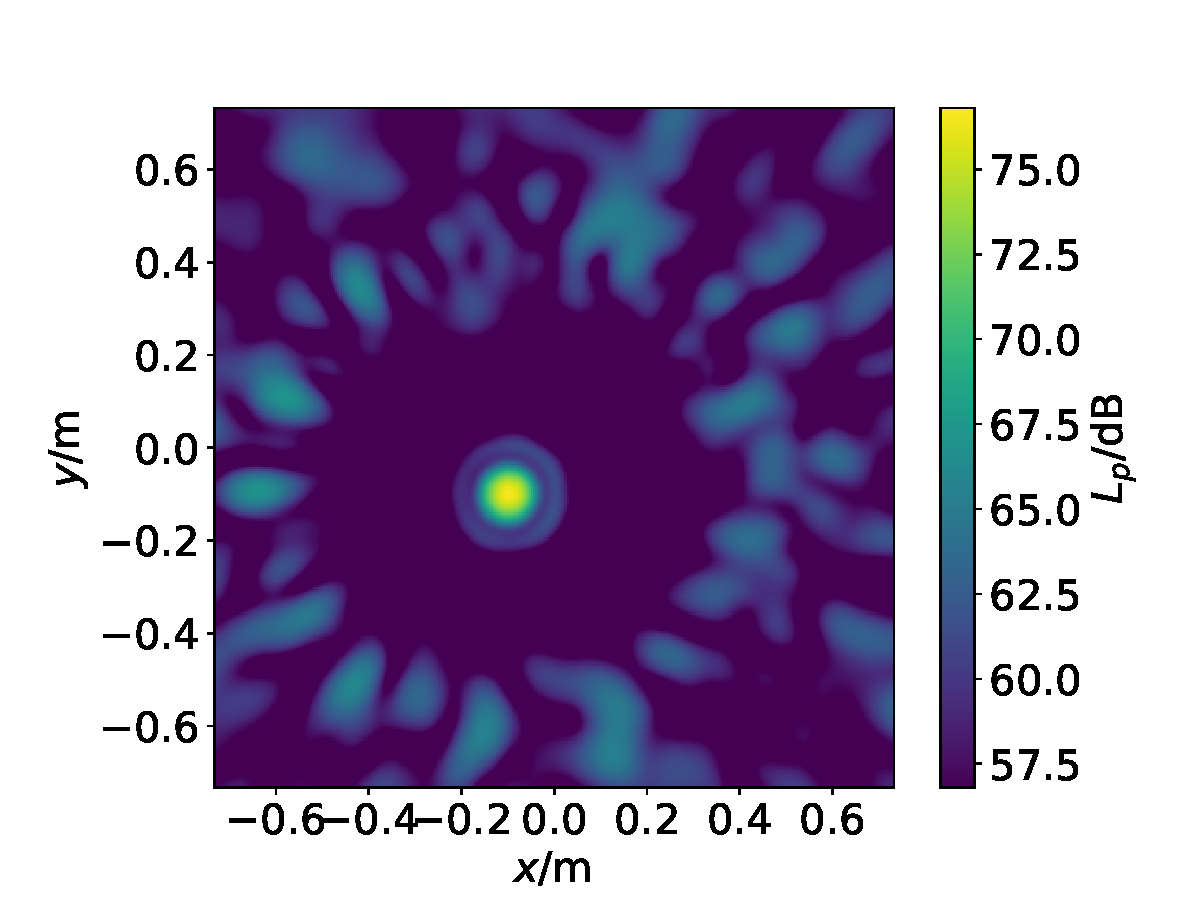
\includegraphics[width=0.75\linewidth]{figs/datasets_beamforming_example_measurement.pdf} 
      \caption{Measurement}
      %\label{fig7:b} 
      %\vspace{4ex}
    \end{subfigure}
  \end{figure}
  
\end{psli}

\begin{psli}[Methods: Generating Eigenvalues]  
    The first approach consisted in generating the scaled eigenvalues $[\lambda_0, \dots, \lambda_{63}] \in ]0,1]^{64}$, with $\lambda_0 \leq \lambda_1 \leq \dots \leq \lambda_{63}$. This approach allowed to scale generated eigenavalues, before feeding them to the discriminator, in order to improve performances.


    \begin{table}[h]
      \centering
      \begin{minipage}[b][0.5\textheight][b]{0.45\textwidth}
        %\centering
        \resizebox{\columnwidth}{!}{
        \begin{tabular}{c c c}
            \hline
            \textbf{Layer} & \textbf{Output Shape} & \textbf{Number of Parameters} \\ \hline
            InputLayer            & 128           & 0                 \\ 
            Dense                 & 256           & 32768             \\ 
            LeakyReLU             & 256           & 0                 \\ 
            BatchNormalization    & 256           & 1024              \\ 
            Dense                 & 512           & 131584            \\ 
            LeakyReLU             & 512           & 0                 \\ 
            Dense                 & 1024          & 525312            \\ 
            LeakyReLU             & 1024          & 0                 \\ 
            Dense                 & 64            & 65600             \\ 
        \end{tabular}
        }
        \caption{Generator}
      \end{minipage}
      \begin{minipage}[b][0.5\textheight][b]{0.45\textwidth}
        %\centering
        \resizebox{\columnwidth}{!}{%
        \begin{tabular}{c c c}
            \hline
            \textbf{Layer} & \textbf{Output Shape} & \textbf{Number of Parameters} \\ \hline
            InputLayer            & 64            & 0                 \\
            Dense                 & 512           & 33280             \\
            LeakyReLU             & 512           & 0                 \\
            Dense                 & 256           & 131328            \\
            LeakyReLU             & 256           & 0                 \\
            Dense                 & 1             & 257               \\
        \end{tabular}
        }
        \caption{Discriminator}
      \end{minipage}
    \end{table}
\end{psli}

\begin{psli}[Methods: Generating Eigenvalues]
  
    The second approach to generate the eigenvalues consisted in generating their level representation $L_{\lambda_0}, \dots, L_{\lambda_{63}}$ defined as:
    \begin{equation}
        L_{\lambda_i} = 10 \log_{10}(\frac{\lambda_i}{\lambda_{63}})
    \end{equation}
    %Since all values $L_{\lambda_i}$ are non-positive, the generator has been built such that the two last steps are first a ReLU, followed by a multiplication by $-1$. This way it can be ensured that the network only produces non-positive spectrum. This approach was also justified by the usage of Leaky ReLU as activation throughout the generator. Because Leaky ReLU were used in the critic, the first layer of its network is also a multiplicative layer. %Therefore, the critic is not trained to detect real from fake levels, but rather real from fake negative levels, which is equivalent.

    \begin{table}[h]
      \centering
      \begin{minipage}[b][0.3\textheight][t]{0.45\textwidth}
          %\centering
          \resizebox{\columnwidth}{!}{
            \begin{tabular}{c c c}
              \hline
              \textbf{Layer} & \textbf{Output Shape} & \textbf{Number of Parameters} \\ \hline
              InputLayer            & 128           & 0                 \\
              Dense                 & 256           & 32768             \\
              LeakyReLU             & 256           & 0                 \\
              BatchNormalization    & 256           & 1024              \\
              Dense                 & 512           & 131584            \\
              LeakyReLU             & 512           & 0                 \\
              Dense                 & 1024          & 525312            \\
              LeakyReLU             & 1024          & 0                 \\
              Dense                 & 64            & 65600             \\
              ReLU                  & 64            & 0                 \\
              Multiply              & 64            & 0                 \\
          \end{tabular}
          }
          \caption{Generator}
  
      \end{minipage}
      \begin{minipage}[b][0.3\textheight][t]{0.45\textwidth}
          %\centering
          \resizebox{\columnwidth}{!}{%
          \begin{tabular}{c c c}
            \hline
            \textbf{Layer} & \textbf{Output Shape} & \textbf{Number of Parameters} \\ \hline
            InputLayer            & 64            & 0                 \\
            Multiply              & 64            & 0                 \\
            Dense                 & 512           & 33280             \\
            LeakyReLU             & 512           & 0                 \\
            Dense                 & 256           & 131328            \\
            LeakyReLU             & 256           & 0                 \\
            Dense                 & 1             & 257               \\
          \end{tabular}
          }
          \caption{Discriminator}
      \end{minipage}
    \end{table}
   
  
  
\end{psli}

\begin{psli}[Methods: Generating Eigenvectors]
  \begin{itemize}
    \item As a proof of concept, it was decided to start by only generating the strongest eigenvector, defined as main eigenvector.
    \item The main eigenvector contains all the information about the position of the source. %Indeed, each eigenvector belongs to a different incoherent source. If there would to be  multiple coherent source, all the energy and their position merges into a single eigenmode. Since the case where there is only one source is under consideration, only the eigenvector with the biggest index corresponds to a DoA/source and the remaining 63 eigenvectors corresponds to noise.
    %\item Since the main eigenvector is $\in \mathbb{C}^{64}$, a network with a similar architecture as the one used for the eigenvalues can be used. But instead of scaling the generated sample, they are normalized before being fed to the discriminator. %Here by normalization is meant that the main eigenvector is recomputed such that its direction remains the same but its norm is equal to 1.  
  \end{itemize}

  \begin{table}[h]
    \centering
    \begin{minipage}[b][0.3\textheight][t]{0.45\textwidth}
        %\centering
        \resizebox{\columnwidth}{!}{
          \begin{tabular}{c c c}
            \hline
            \textbf{Layer} & \textbf{Output Shape} & \textbf{Number of Parameters} \\ \hline
            InputLayer            & 128           & 0                 \\
            Dense                 & 256           & 32768             \\
            LeakyReLU             & 256           & 0                 \\
            BatchNormalization    & 256           & 1024              \\
            Dense                 & 512           & 131584            \\
            LeakyReLU             & 512           & 0                 \\
            Dense                 & 1024          & 525312            \\
            LeakyReLU             & 1024          & 0                 \\
            Dense                 & 128           & 131200            \\
            Reshape               & (1, 64, 2)    & 0                 \\
          \end{tabular}
        }
        \caption{Generator}

    \end{minipage}
    \begin{minipage}[b][0.3\textheight][t]{0.45\textwidth}
        %\centering
        \resizebox{\columnwidth}{!}{%
        \begin{tabular}{c c c}
          \hline
          \textbf{Layer} & \textbf{Output Shape} & \textbf{Number of Parameters} \\ \hline
          InputLayer            & (1, 64, 2)    & 0                 \\
          Flatten               & 128           & 0                 \\
          Dense                 & 512           & 66048             \\
          LeakyReLU             & 512           & 0                 \\
          Dense                 & 256           & 131328            \\
          LeakyReLU             & 256           & 0                 \\
          Dense                 & 1             & 257               \\
        \end{tabular}
        }
        \caption{Discriminator}
    \end{minipage}
  \end{table}
\end{psli}

\begin{psli}[Methods: Data Augmentation]
  
  For a received synthetic CSM $\mathbf{\hat{C}}$, its  eigendecomposition $\mathbf{\hat{C}} = \mathbf{V} \mathbf{\Lambda} \mathbf{V}^H$ is computed. The CSM $\mathbf{\hat{C}}$ can then be modified with
  
  \begin{itemize}
    \item generated eigenvalues $\hat{\mathbf{\Lambda}}$, with:
    \begin{equation}
        \mathbf{\hat{C}}_\text{augm.}^{\mathbf{\Lambda}}  = \mathbf{V} \hat{\mathbf{\Lambda}} \mathbf{V}^H
    \end{equation}

    \item a generated main eigenvector $\hat{\mathbf{v}}_M$ and corresponding semi-generated eigenvectors matrix $\hat{\mathbf{V}} = [\mathbf{v}_1^T, \dots, \hat{\mathbf{v}}_M^T]$, with:

    \begin{equation}
        \mathbf{\hat{C}}_\text{augm.}^{\mathbf{V}}  = \hat{\mathbf{V}} \mathbf{\Lambda} \hat{\mathbf{V}}^H
    \end{equation}

  \end{itemize}

\end{psli}

\begin{psli}[Results and Discussion: Generating eigenvalues from scaled values]
  \begin{minipage}[b][0.7\textheight][t]{0.5\textwidth}
    \centering
    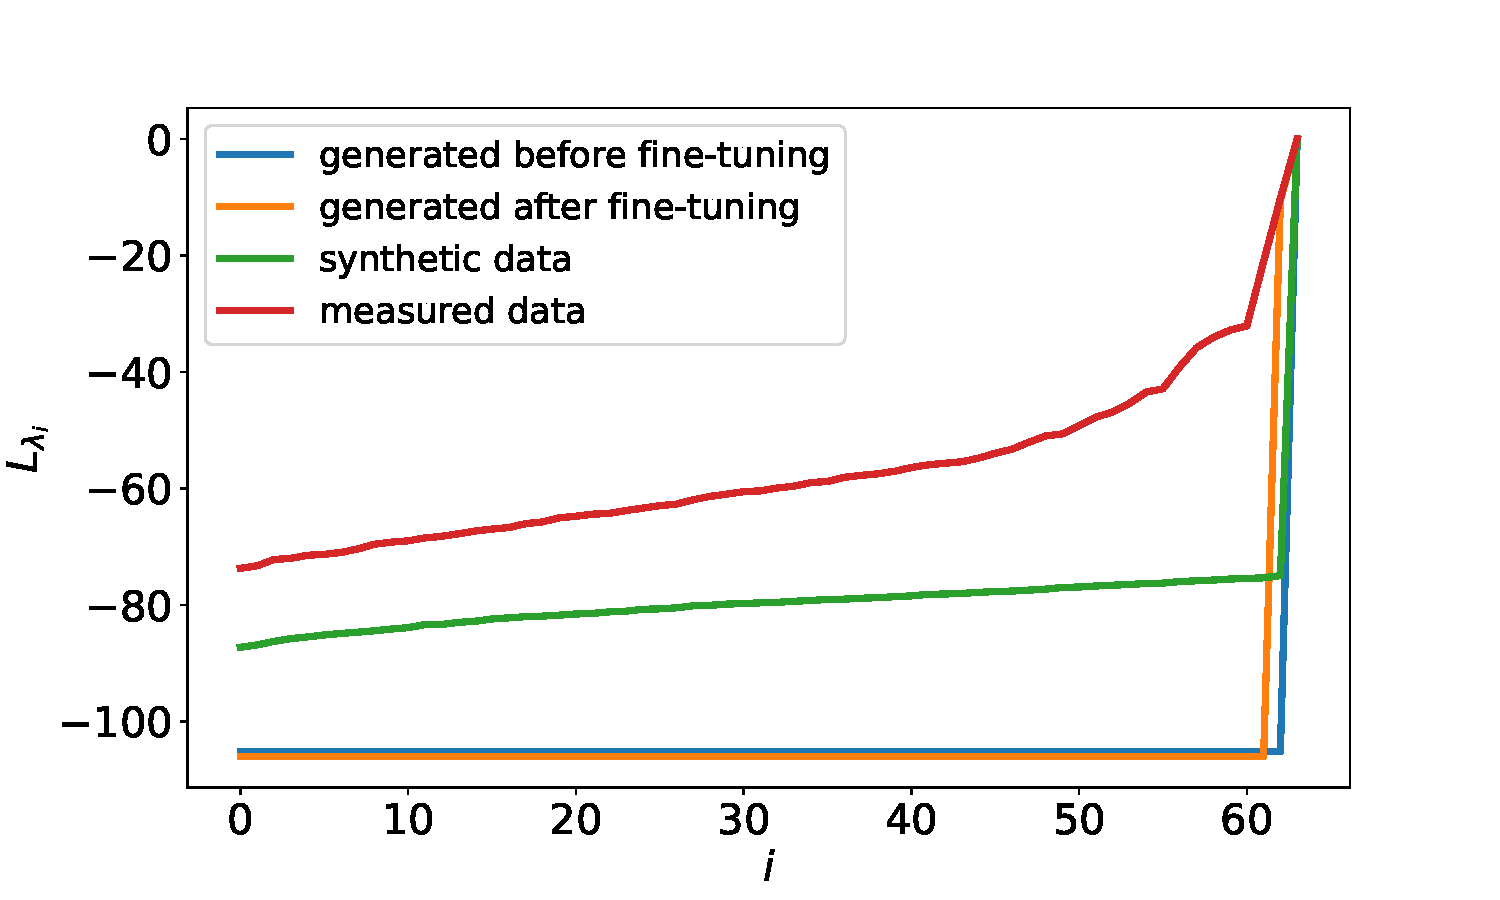
\includegraphics[width=1.2\textwidth]{figs/samples_evals_wgangp.pdf}
  \end{minipage}
  \begin{minipage}[b][0.7\textheight][t]{0.5\textwidth}
    \begin{itemize}
        \item Sudden and steep drop in value, reaching a level around $10^{-100}$, both before and after fine-tuning.
        \item the WGAN-GP cannot capture very well small numerical variation.
        \item This approach is not suited.
    \end{itemize}
  \end{minipage}
\end{psli}

\begin{psli}[Results and Discussion: Generating eigenvalues from levels]
  \begin{minipage}[b][0.7\textheight][t]{0.5\textwidth}
    \centering
    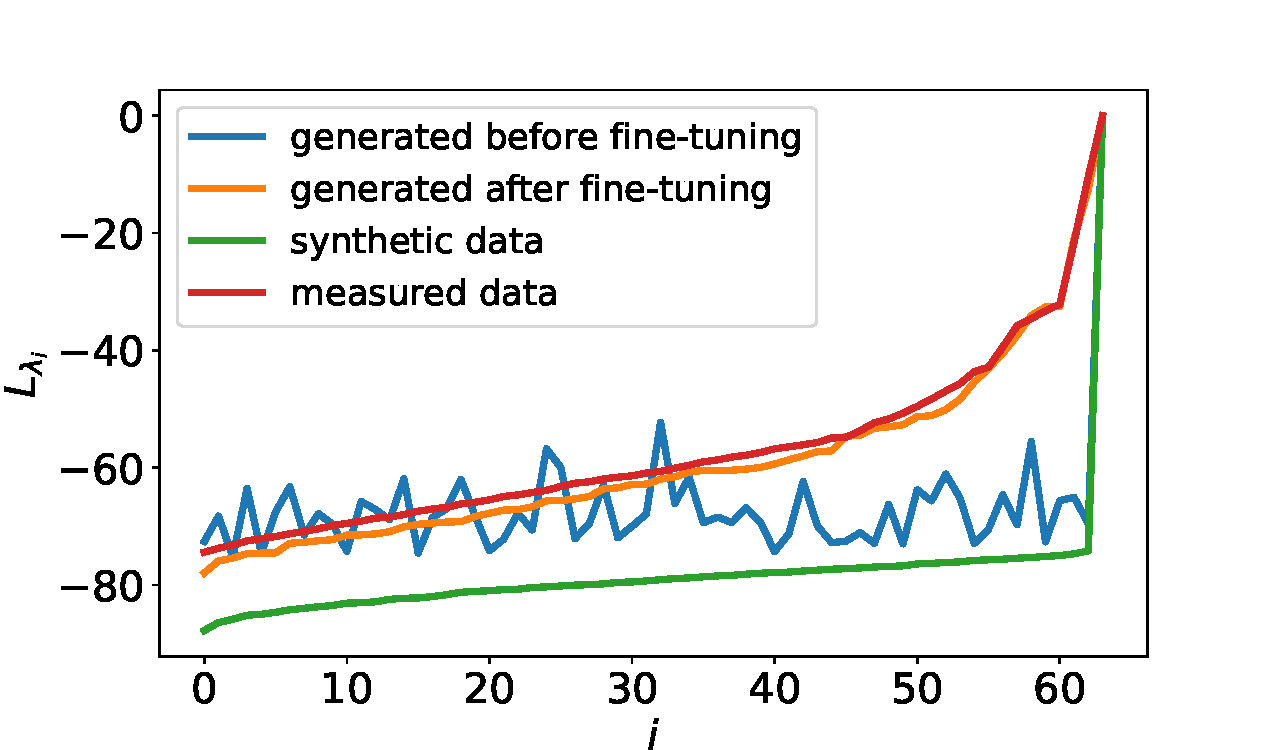
\includegraphics[width=1.2\textwidth]{figs/samples_evals_dB_wgangp.pdf}
  \end{minipage}
  \begin{minipage}[b][0.7\textheight][t]{0.5\textwidth}
    \begin{itemize}
        \item The generated data looks more like the real data, especially after fine-tuning.
        \item Generating the eigenvalues from their levels produces satisfying results.
    \end{itemize}
  \end{minipage}
\end{psli}

\begin{psli}[Results and Discussion: Generating eigenvalues from levels 2]
  \begin{minipage}[b][0.7\textheight][t]{0.5\textwidth}
    \centering
    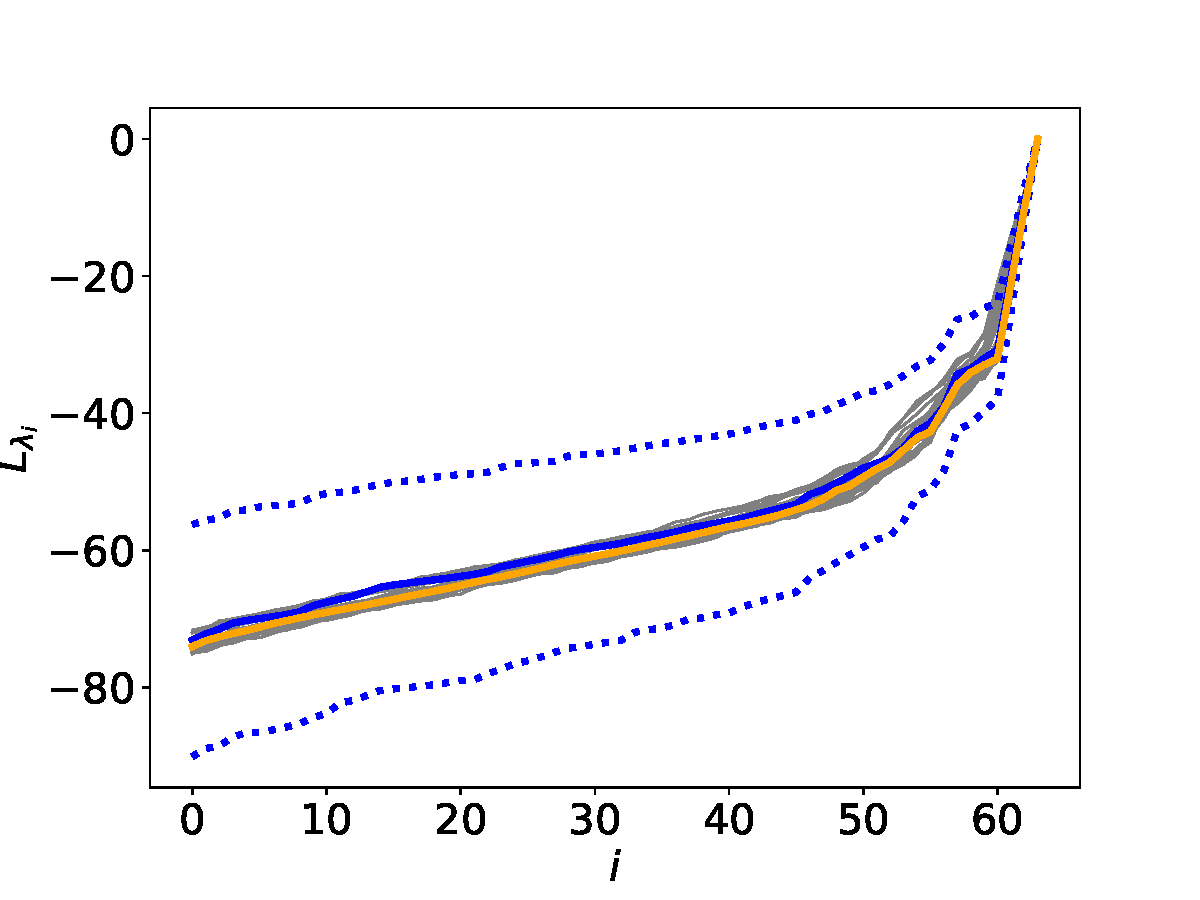
\includegraphics[width=1.2\textwidth]{figs/outliers_evals_dB_wgangp.pdf}
  \end{minipage}
  \begin{minipage}[b][0.7\textheight][t]{0.5\textwidth}
    \begin{itemize}
        \item Training the network first with synthetic data and then fine-tuning it with a single measurement allows to produce eigenvalues with a large variation.
        \item This approach allows to generate eigenvalues samples that are representative not only of a single measurement, but of multiple ones.
    \end{itemize}
  \end{minipage}
\end{psli}



\begin{psli}[Results and Discussion: Generating strongest eigenvector]
  
    \begin{minipage}[t][0.3\textheight][t]{0.4\textwidth}
      \centering
      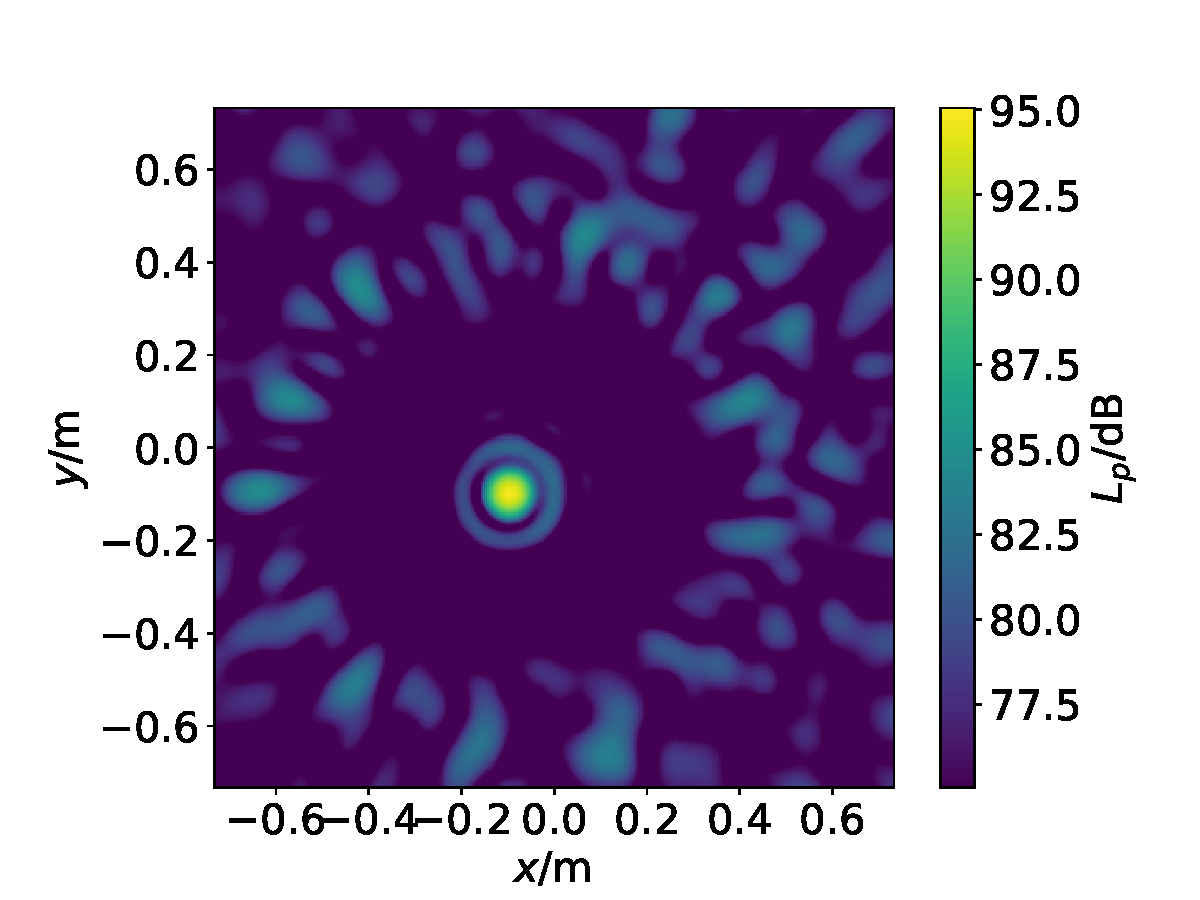
\includegraphics[width=1.2\textwidth]{figs/beamforming_map_main_evec_wgangp_generated.pdf}
    \end{minipage}
    \begin{minipage}[b][0.7\textheight][t]{0.5\textwidth}
      \begin{itemize}
          \item The beamforming map computed from a Rank I CSM with generated main eigenvector is sufficiently realistic sample.
          \item It was observed that all the generated main eigenvector were similar.
          \item the WGAN-GP cannot produce a great variety of sample, but it is representative of the data it was trained with.  
      \end{itemize}
    \end{minipage}
  \end{psli}


% ============================================================
\begin{psli}[Results and Discussion: Data Augmentation]
  \begin{figure}
    \begin{subfigure}[b]{0.45\linewidth}
      \centering
      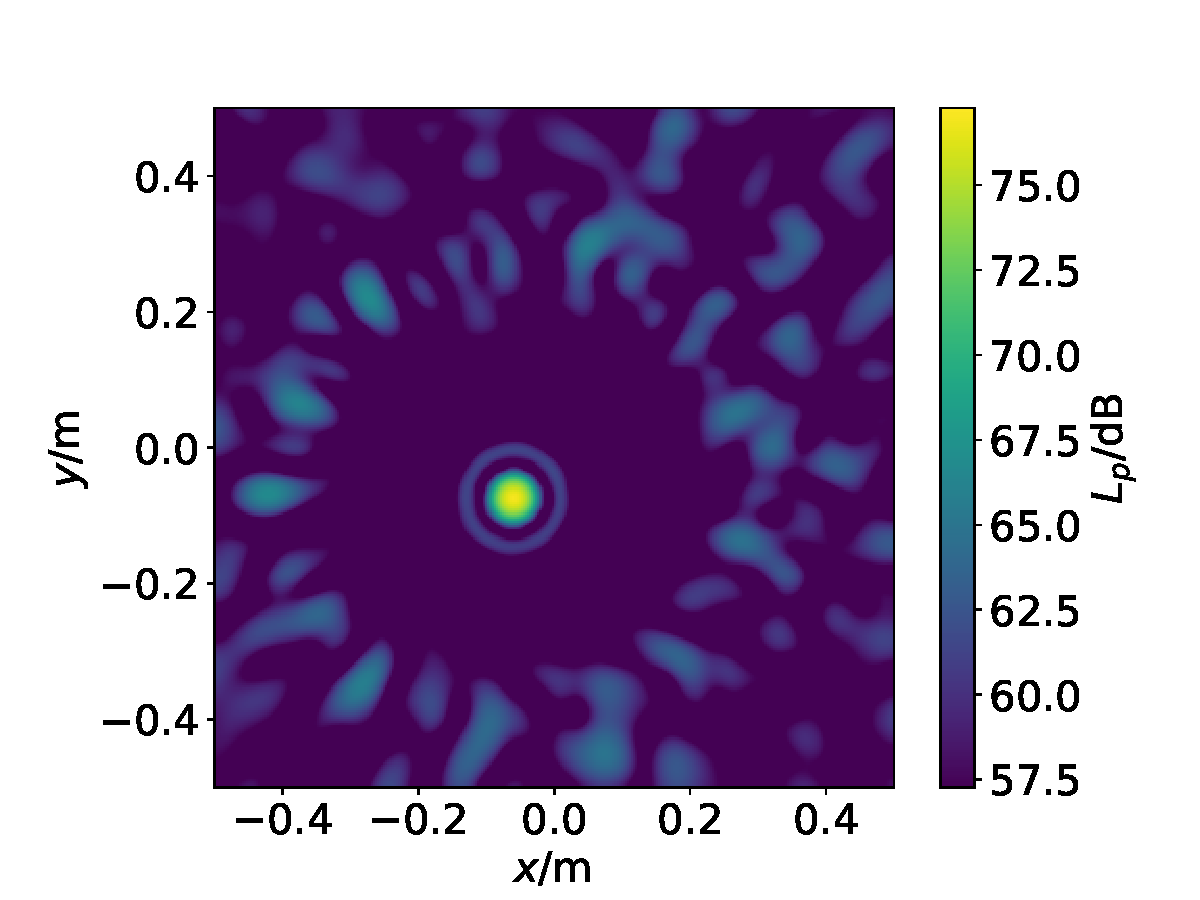
\includegraphics[width=0.5\linewidth]{figs/datasets_beamforming_example_synthetic.pdf} 
      \caption{Synthetic} 
      %\label{fig7:a} 
      %\vspace{4ex}
    \end{subfigure}%% 
    \begin{subfigure}[b]{0.45\linewidth}
      \centering
      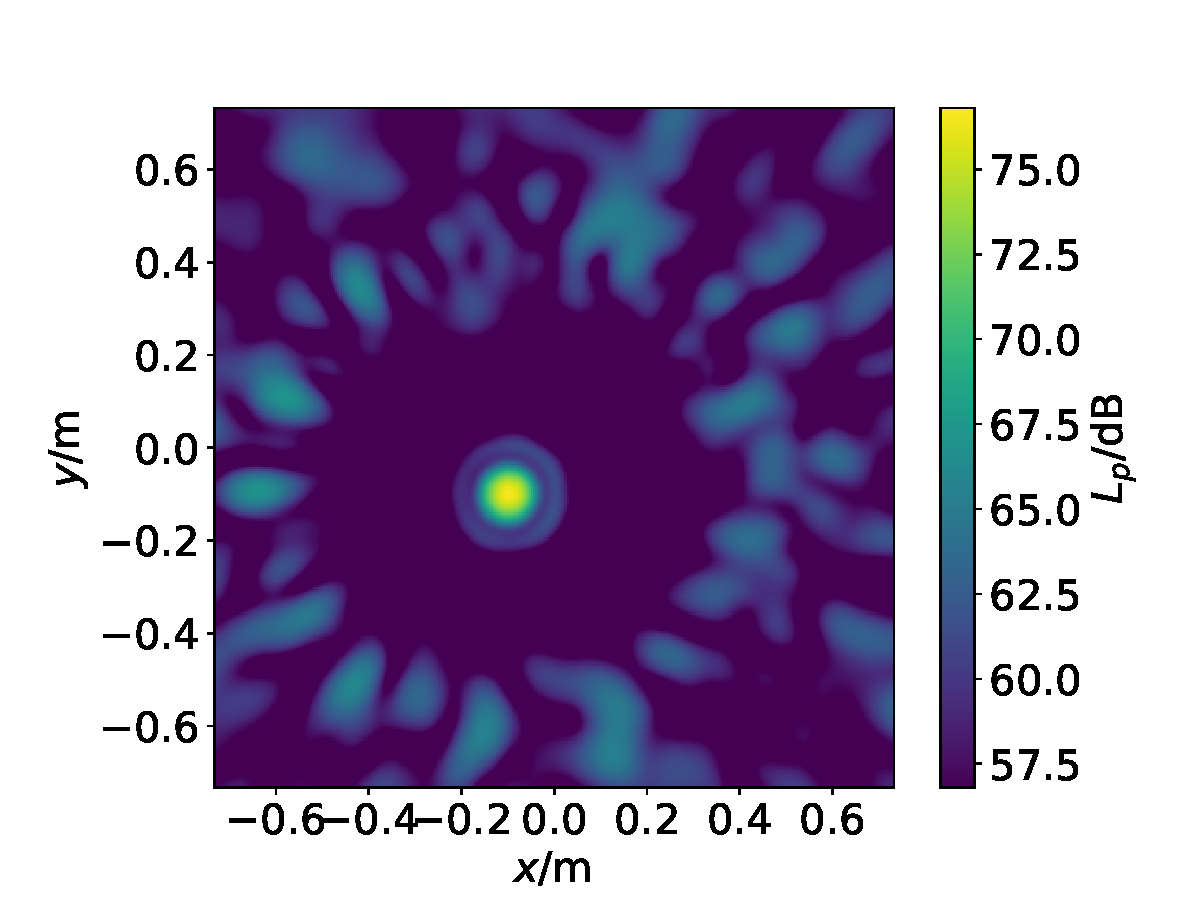
\includegraphics[width=0.5\linewidth]{figs/datasets_beamforming_example_measurement.pdf} 
      \caption{Measurement} 
      %\label{fig7:b} 
      %\vspace{4ex}
    \end{subfigure} 
    \begin{subfigure}[b]{0.45\linewidth}
      \centering
      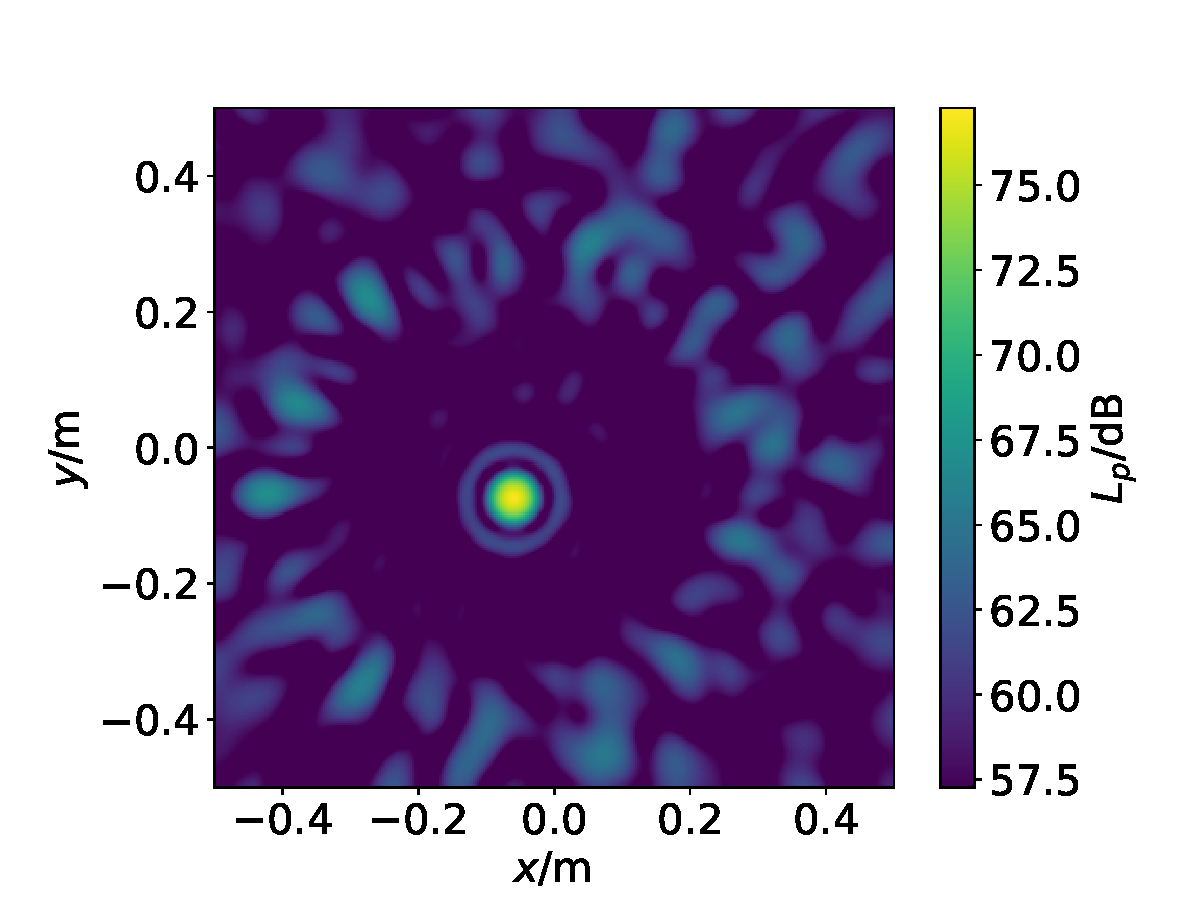
\includegraphics[width=0.5\linewidth]{figs/data_augmentation_evals_augmented_csm.pdf} 
      \caption{Augmented with Eigenvalues} 
      %\label{fig7:c} 
    \end{subfigure}%%
    \begin{subfigure}[b]{0.45\linewidth}
      \centering
      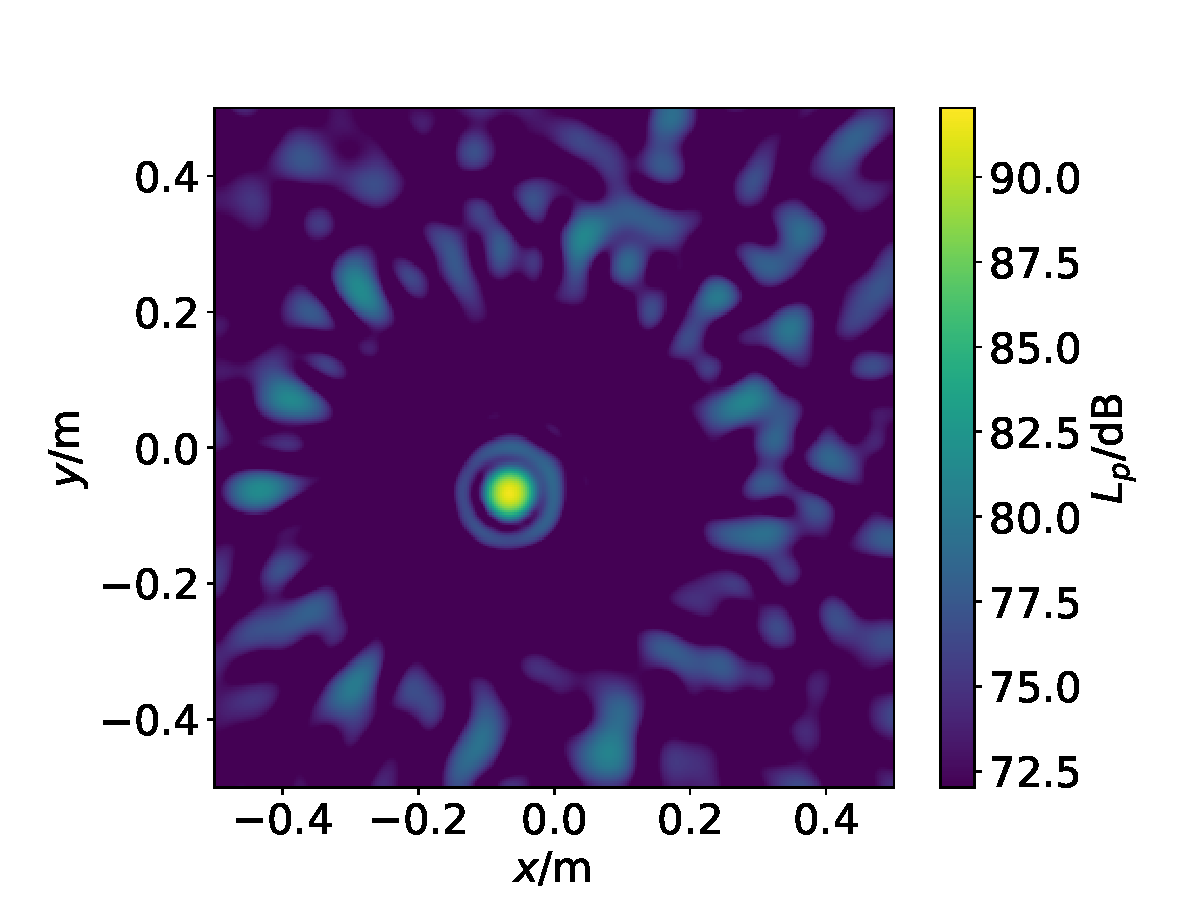
\includegraphics[width=0.5\linewidth]{figs/data_augmentation_evecs_augmented_csm.pdf} 
      \caption{Augmented with Eigenvectors}  
    \end{subfigure} 
  \end{figure}
\end{psli}
% ============================================================

\begin{psli}[Conclusion]
  \begin{itemize}
    \item WGAN-GPs are suited to generate eigenvalues and strongest eigenvector. 
    \item The data augmentation methods introduced allow to improve how realistic synthetic CSM are.
    \item The eigedecomposition is a good representation of CSM to learn their distribution. 
    \item The finding in this thesis are an important step toward solving the unavailability of real training data for source localization or characterization. 
  \end{itemize}
\end{psli}

\begin{psli}[Future Works]
  \begin{itemize}
    \item Extending the work to be able to generate CSM for different positions. 
    %\item More specifically, this would need to be done for the network to generate the main eigenvector. Indeed, the eigenvalue spectrum is not position dependent.
    \item Investigate whether a Neural Network could be designed for generating eigenvectors corresponding to a given source position not observed in the dataset.
    %It is to be noted that a good starting point for this investigation would be to attempt to build a Neural Network to learn relationship between source position and the main eigenvector.
    
    \item Investigate how to generate the remaining weakest eigenvectors. 
  \end{itemize}
\end{psli}

\begin{psli}
  \begin{center}
      Questions? 
  \end{center}
\end{psli}

\begin{psli}[Bibliography]
  % Bibliography
  \bibliographystyle{IEEEtran} % bibliography style in order of first citation
  \bibliography{./resources/IEEEabrv,./bibliography}
\end{psli}

\begin{psli}[Appendix: loss function WGAN-GP to generate eigenvalues from scaled values]
  \centering
  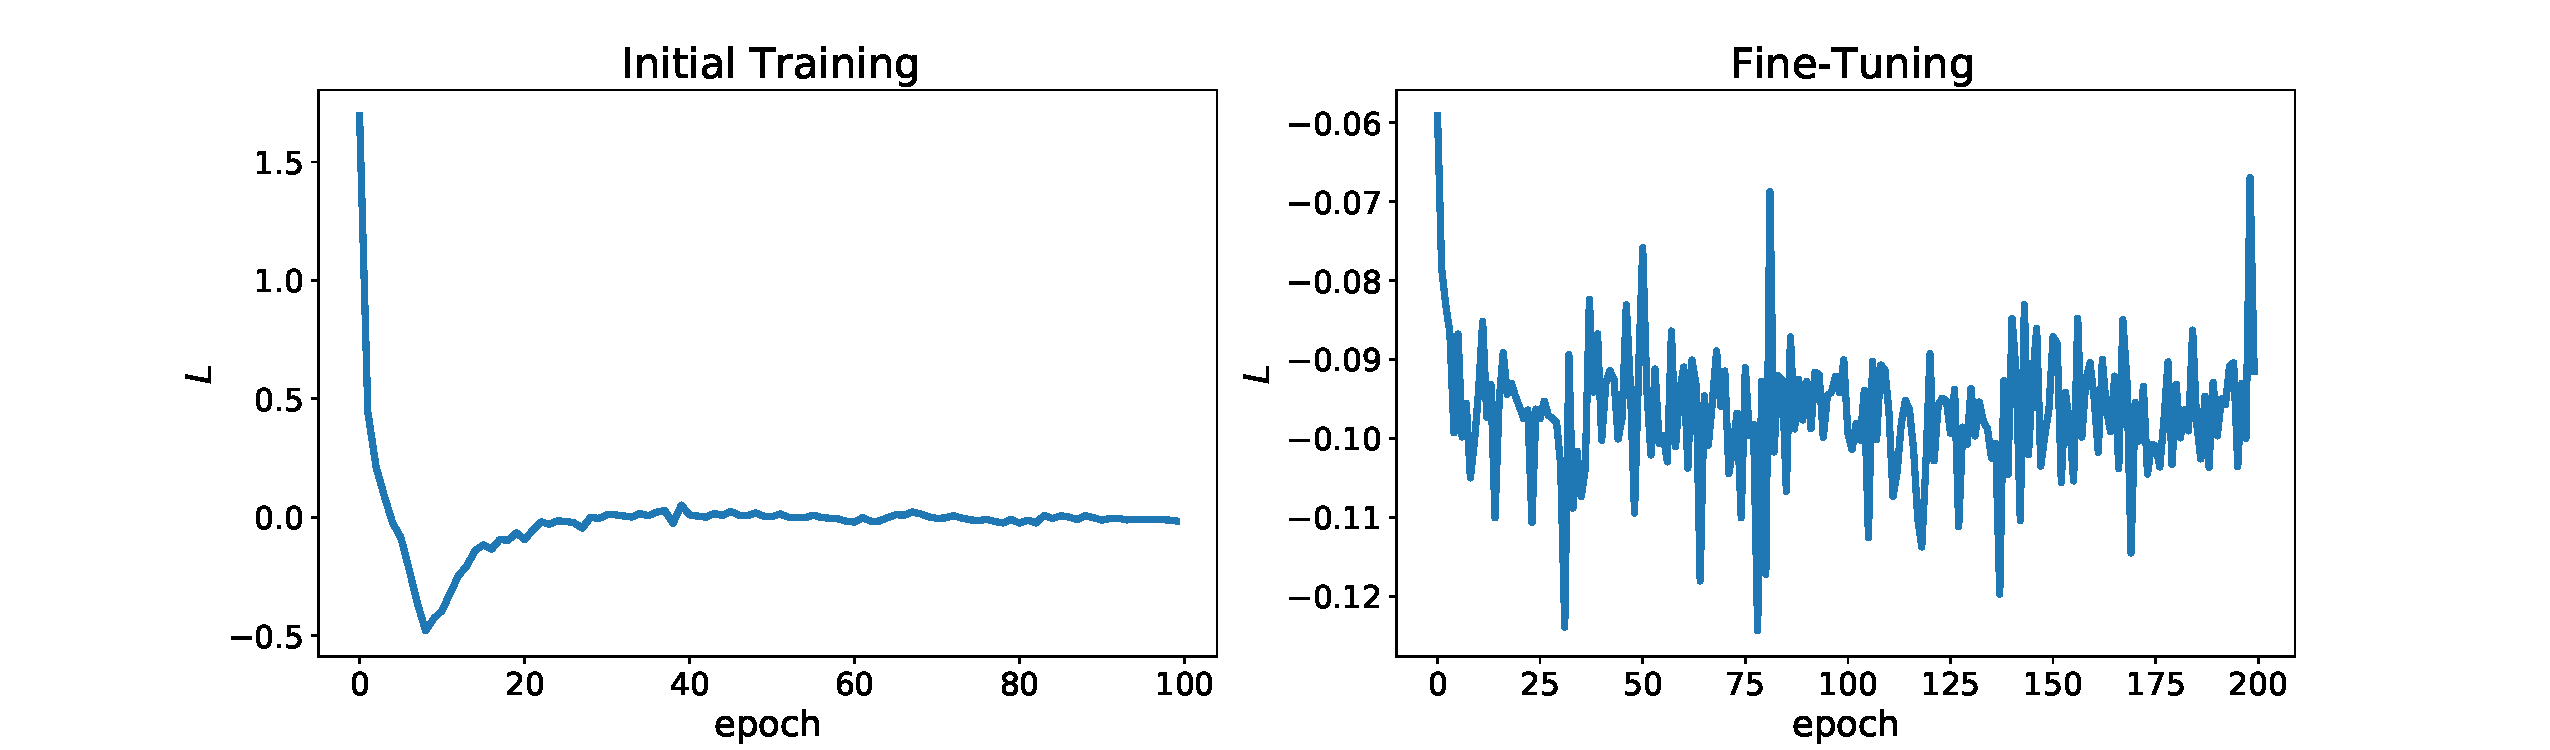
\includegraphics[width=1\textwidth]{figs/loss_evals_wgangp.pdf}
\end{psli}

\begin{psli}[Appendix: loss function WGAN-GP to generate eigenvalues from level]
  \centering
  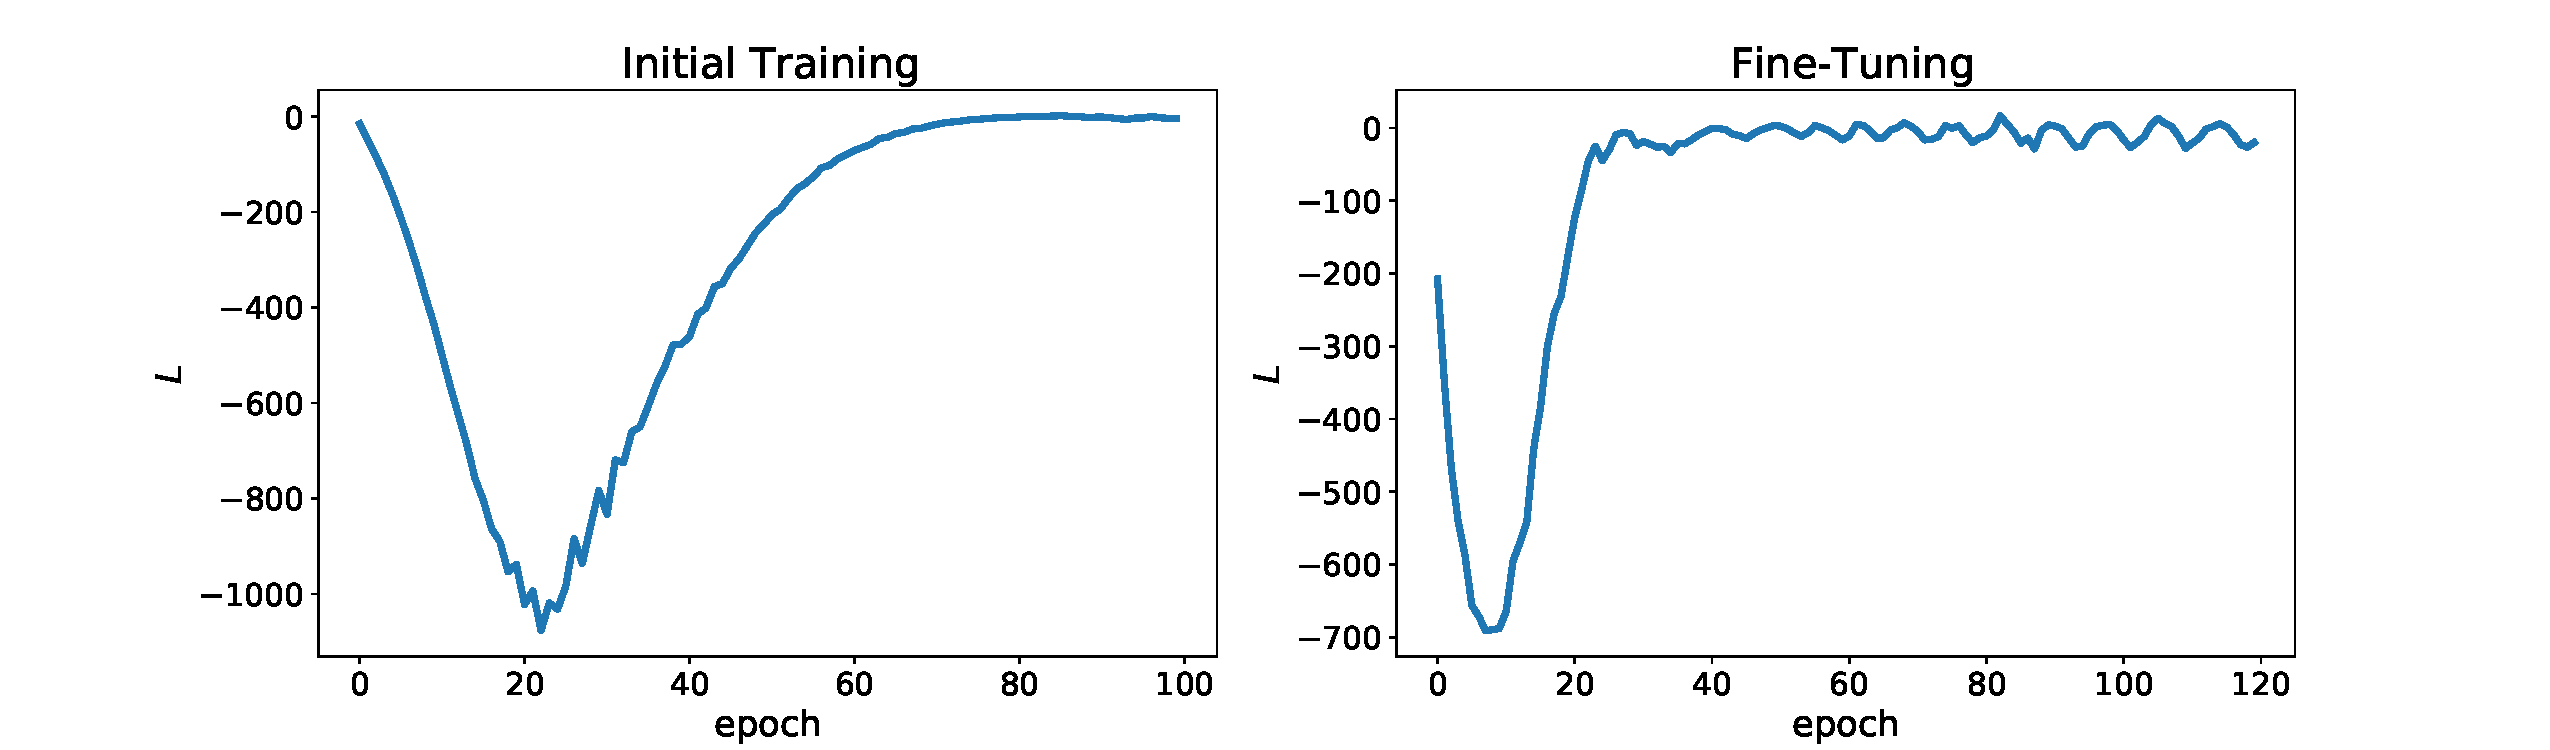
\includegraphics[width=1\textwidth]{figs/loss_evals_dB_wgangp.pdf}
\end{psli}

\begin{psli}[Appendix: loss function WGAN-GP to generate main eigenvector]
  \centering
  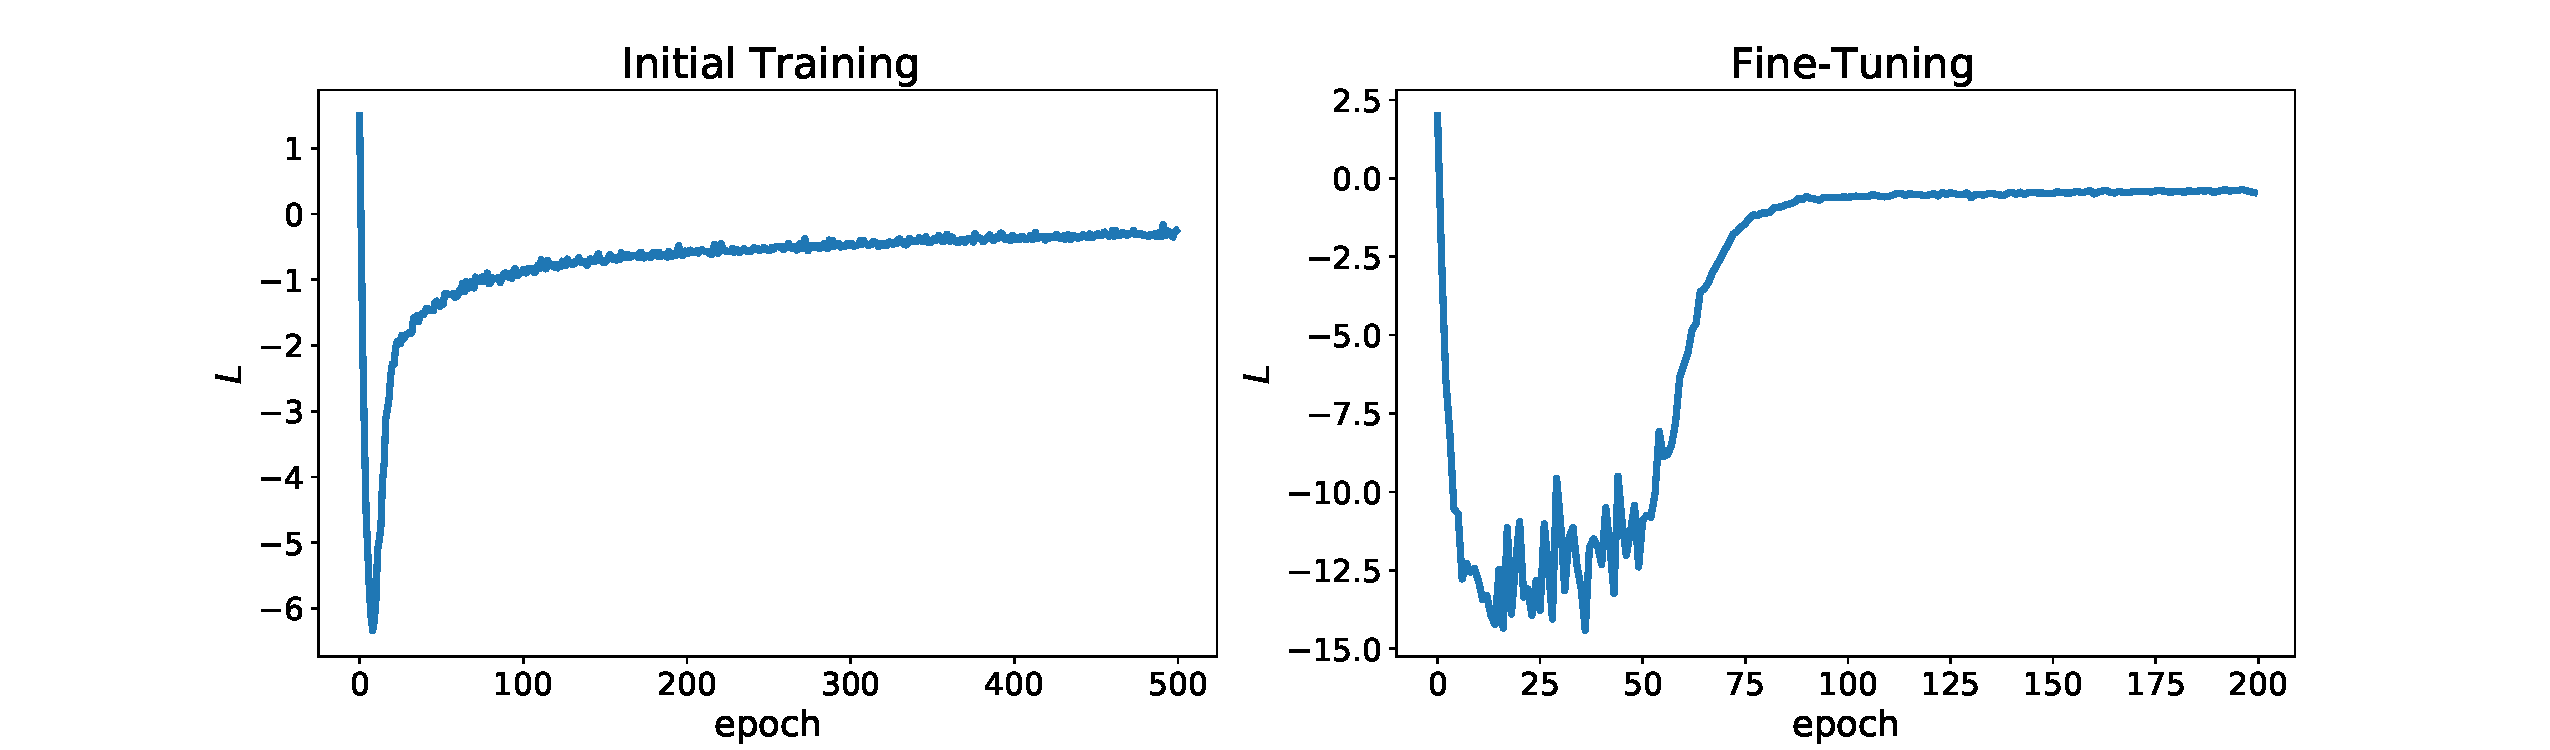
\includegraphics[width=1\textwidth]{figs/loss_main_evec_wgangp.pdf}
\end{psli}



\end{document}

%%% Local Variables:
%%% mode: latex
%%% TeX-master: t
%%% End:
